%---------------------------------------------------------------------------------------------%
\section{Network Virtualization}

Network virtualization has gained an extreme importance in data center networking
as it enables cloud providers to enhance the flexibility, scalability 
and resource utilization of the network infrastructure. Multiple virtual 
networks can be deployed on a single physical infrastructure with 
network virtualization. 

In this section, we first explain what network virtualization is and how it is 
different from the conventional non-virtualized envrionments 
(Section \ref{sec:nonvirt.vs.virt}). We then explore different network virtualization
platforms and investigate their shortcommings in providing network virtualization 
for low-latency and high-throughput data center applications (Section \ref{sec:network.virt.platform}).


\subsection{Non-virtualized vs. virtualized network environments}
\label{sec:nonvirt.vs.virt}

\begin{figure}
    \centering
    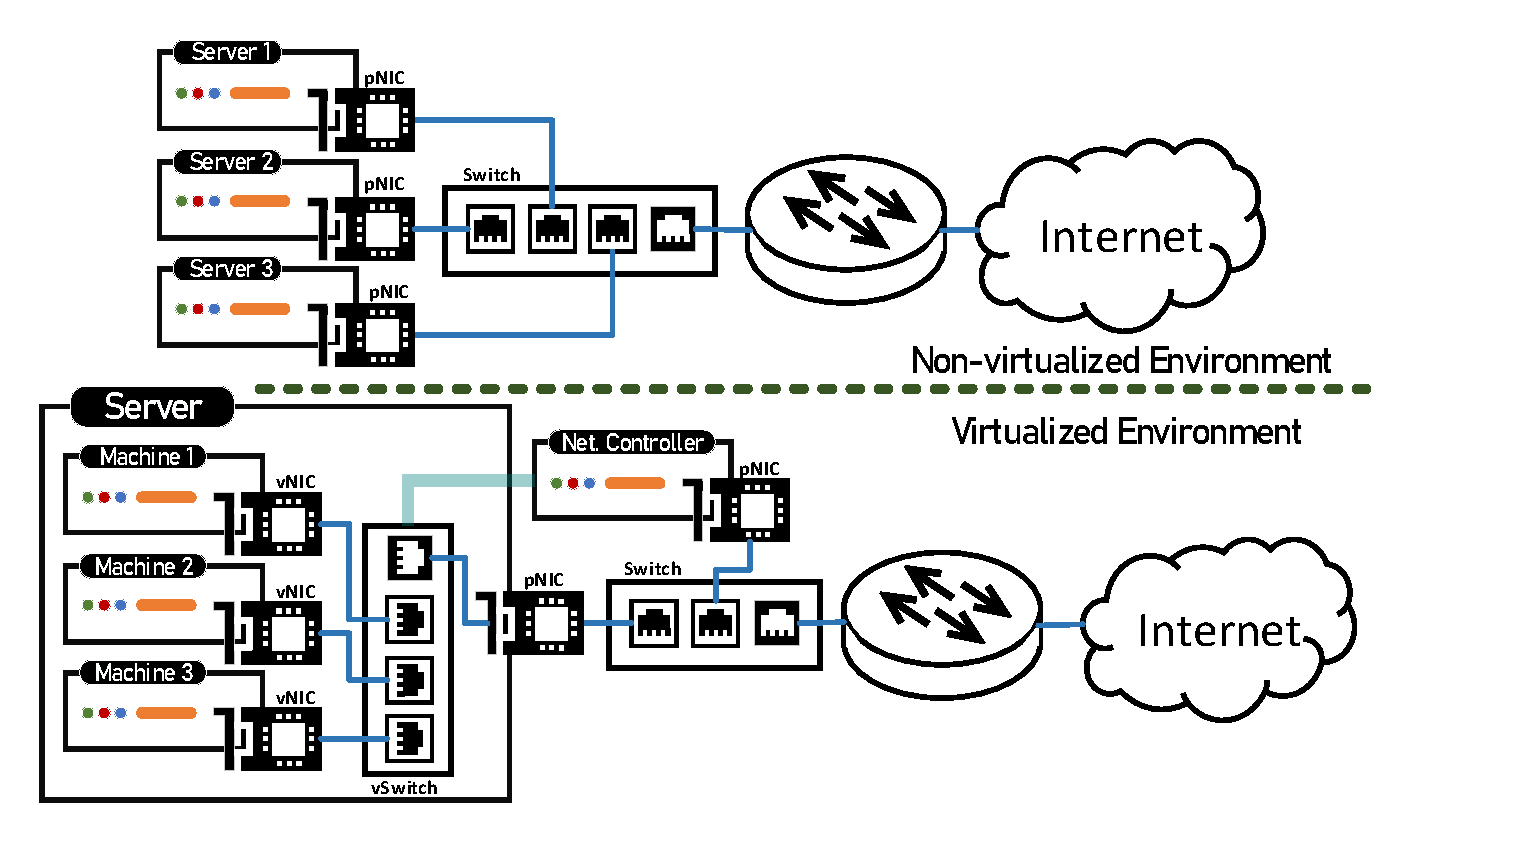
\includegraphics[scale=0.625]{../Figures/non-virt-vs-virt.pdf}
    \caption{Non-virtualized vs. virtualized network environment}
    \label{fig:overhead.throughput}
\end{figure}



In a non-virtualized network environment, networking components are directly tied 
to the underlying physical hardware. Each network component, such as a switch or router, 
corresponds to a specific physical device, and the network as a whole is limited by the 
available hardware resources. This makes configuration a hard and 
time-consuming task. Each networking vendor has its own interface, and configuring each 
device requires the corresponding expertise. In addition to that, adding or removing a machine 
requires multiple configurations to be set up in a box-by-box manner, which introduces 
an excessive operation overhead and increases the risk of misconfiguration 
\cite{cearley2013top, marty2019snap}.

Network virtualization aims to solve these issues by separating and abstracting 
network configuration from the underlying hardware.
Through a virtualization layer, users can create virtual networks, with arbitrary service 
models, topologies, and addressing scheme, on top of the same physical network devices. Furthermore, 
a global abstraction enables management and configuration of these virtual networks 
\cite{mckeown2008openflow}.


\subsection{Network virtualization platforms}
\label{sec:network.virt.platform}

To provide network virtualization for cloud tenants, public cloud providers, such as Amazon 
Web Services (AWS), Microsoft Azure, and Google Cloud Platform (GCP), have taken different 
approaches. While Microsoft has been following a hardware-assisted procedure to provision 
networking demands \cite{firestone2018azure, firestone2017vfp}, Google has been utilizing 
a software-only approach \cite{marty2019snap}. In this section, we first introduce two seminal 
open-source projects in network virtualization, namely OpenFlow (Section \ref{OpenFlow}), 
and Open Virtual Switch (Section \ref{OVS}). We then elaborate on the state-of-the art network 
virtualization used by VMWare (Section \ref{nvp}), Google (Section \ref{snap}), and 
Microsoft(Section \ref{vfp}).

\subsection{OpenFlow}
\label{OpenFlow}
\textbf{OpenFlow} was first proposed to enhance the implementation of new protocols on top 
of the production networks. It consists of a standardized interface to add or remove entries 
from flow tables residing on the Ethernet switches \cite{mckeown2008openflow}.

Flow tables are the fundamental data structure of an OpenFlow switch. They consist of flow 
entries and proper actions to the packets of each flow. A flow is a set of packets that have 
similar characteristics. It could be a TCP connection, all packets from a particular port 
number, or packets with the same VLAN tag. An OpenFlow switch matches the packets with the 
specified flows and applies the action of that flow. For example, all packets from a 
particular sender could be dropped by the OpenFlow switch. 

The three basic actions that are supported by an OpenFlow switch consists of (\emph{i}) 
forwarding packets to a given port (or ports), (\emph{ii}) encapsulating and forwarding 
packets to a controller, and (\emph{iii}) dropping packets.


In summary, an OpenFlow switch has the following three main components:
\begin{enumerate}
    \item \emph{A Flow-table residing on the Ethernet switch}: This flow table maintains 
    information about existing flows and actions required to be applied to the corresponding 
    packets.
    \item \emph{Secure interface between a controller and the switch}: The interface is used 
    when a packet has no corresponding entry in the flow table. In such scenarios, the packets 
    will be forwarded through this interface to a controller. The controller can then decide 
    for the corresponding action.
    \item \emph{Standardized OpenFlow interface to program flow tables}: With this standardized
    interface, a controller can update the flow-tables on Ethernet switches. Therefore, not 
    all the packets are required to be transferred to the controller, hence higher throughput 
    can be achieved. 
\end{enumerate}

Further detailed specifications of an OpenFlow switch are defined by 
\emph{Open Networking Foundation} \cite{specification2009version}. 

VirtTAS supports OpenFlow interface to enable network programmability at end-host.

\subsection{Open Virtual Switch (OVS)}
\label{OVS}

Conventional virtual switches are concerned only with providing a basic network connection 
for VMs through L2 networks. This was changed with the advent of network virtualization. 
Today's virtual switches provide most network services for VMs, and the physical networks 
only transmit IP-tunneled packets. Therefore, VMs are no longer tightly connected to physical 
datacenter networks and the workloads benefit from higher scalability and mobility.

As the complexity of network virtualization increased, the need for a production-level 
multi-layer virtual switch became a necessity. Open vSwitch (OVS) was designed and implemented 
to address this need. It enables network virtualization through OpenFlow and supports standard 
interface management protocols such as NetFlow\cite{claise2004cisco}, sFlow\cite{wang2004sflow}.

Open vSwitch has a long history of development and in order to keep up with the production 
workloads and increase the development velocity, the following key design choices were made 
by OVS community:

\begin{enumerate}
    \item \textbf{Use tuple search classification.}.  Tuple search classification supports 
    constant time updates. Constant time updates are essential in virtualized environments,
    where a controller sends flow updates multiple times a second. Furthermore, it consumes 
    memory linear in the number of flows, and it can be generalized to all combinations of 
    packet header fields.

    \item \textbf{Split implementation between Kernel and userspace.} Kernel-based networking 
    makes the development and release cycles lengthy. Moreover, OVS would not be accepted as 
    a contribution to upstream Linux, if it was implemented solely in Kernel. Thereby, OVS 
    uses kernel as a match and action cache and the main classification labor is done in 
    userspace by a virtual switch daemon.

    \item \textbf{Benefit from caching.} OVS uses a two-layers caching mechanism to match 
    packets in the Kernel. A Microflow cache layer matches on specific flows with exact 
    headers fields, and a Megaflow cache layer matches on a wildcard of flows. These wildcards 
    are generated by the cross-product of OpenFlow match and action tables.
    
\end{enumerate}

Although OVS has a positive impact on making virtual switches available for the networking 
community, there are a few shortcomings which makes it not suitable for large scale 
deployments.

\begin{enumerate}
    \item \textbf{Explicit tunnel interface.} OVS uses an extra interface to setup tunneling
    actions, and it hardcodes models of tunneling to dataplane, rather than enabling
    a controller to specify details of tunneling. Therefore, adding complicated tunneling 
    logics, such as ECMP routing, is difficult with OVS. 

    \item \textbf{No support for multi-controller model.} In a multi-controller 
    software-defined network, a virtual switch transmits in-bound packets in the reverse 
    direction of out-bound packets to make the states consistent, whereas OVS only supports forward transmission. 

    \item \textbf{No support for stateful actions} Actions are not stateful, there are 
    trackers supported by OVS but it does not support stateful actions. %TODO polish 

    \item \textbf{Performance} Packets that are not matched in the fast-path cache are 
    handled by the slowpath and in specific cases, these packets are forwarded to a 
    controller. This makes OVS vulnerable to DDoS attacks and cache polution.  %TODO polish 

\end{enumerate}

Despite the limitations of OVS, we decided to integrate OVS into our shared TCP fast-path,
and take the benefits of its long history of development and deployment. Addressing 
the limitations of OVS is beyond the scope of this thesis and we believe the OVS community can
address these issues in the future works. 

\subsection{Network Virtualization Platform (NVP)}
\label{nvp}
Network Virtualization Platform (NVP) is one of the first commercial virtualization 
platform based on SDN that appeared with the market demand for network virtualization
and research on Software Defined Networking (SDN) \cite{koponen2014network}. NVP was proposed 
to address virtualization primitives such as VLAN (Virtualized L2 domain), 
VRFs (Virtualized L3 FIB), NAT 
(Virtualized IP address space), and MPLS (Virtualized Path) needed by VMware's users.

NVP allows users to setup, and configure different virtual networks, each with
different addressing space, independent services model, and topologies
on top of the same physical network. It hides the topology of  the underlaying physical network
from the users, and specific aspects of the forwarding devices becomes unknown for the users. 
In NVP, a hypervisor layer translations each tenant's network configurations to 
low-level instruction set, which can be installed by virtual switches. NVP deploys OVS
as its virtual switch. The packets are tunneled by virtual switches over the physical network, and 
the physical switch only transmit tunneled packets between hypervisors and gateways.

Virt-TAS like NVP, enables virtualization primitivs through use of OVS at end-host. 
NVP, focuses on providing network connectivity to VMs and network programmability 
for operators, whereas Virt-TAS aims to supply VMs with high throughput and low latency 
by streamlining packet processing as a service on hypervisor in addition to providing 
the same features.


\subsection{Google Snap Platform}
\label{snap}

As one of the primary cloud providers with internet-based products that are used by a wide 
range of users, Google has prioritized the following three main requirements for host 
networking in their data centers. 

\begin{enumerate}
    \item \textbf{Fast development and release cycles.} The network bandwidth is continuously 
    increasing and delivering novel approaches for edge switching and bandwidth management is 
    inevitable. Thus, a system that enables fast delivery of innovative paradigms is required.

    \item \textbf{Virtualization features.} Rich virtualization features must be provided on 
    top of host networking to enable cloud computing.

    \item \textbf{Low latency and high throughput.} Distributed data-intensive applications 
    require low latency and high throughput for their communication. As a consequence, the 
    host networking system should be optimized with regard to these applications.

\end{enumerate}

To reach the requirements of data-center networking and to mitigate the drawbacks of using 
the kernel in the development of end-host network stack, Google has proposed Snap. Snap is 
a userspace networking system, which was initially inspired by microkernel architecture. 
By residing in userspace, the development of new features has become faster and upgrades to
the networking stack can be applied transparently. Moreover, in comparison to the Linux Kernel 
networking stack, it provides higher throughput.

\subsection{Virtual Filtering Platform (VFP)}
\label{vfp}

% a paragraph about the overview of VFP
Microsoft Azure has deployed Virtual Filtering Platform (VFP) as its programmable 
virtual switch on more than 1M hosts to provide virtualization features 
\cite{firestone2017vfp}. VFP extends Microsoft Hyper-V's switch 
\cite{hyperv} with the switch logic, and it implements match and actions tables 
with multiple layers to support multi-controller programmability. VFP takes 
advantage of a programming model, which unlike OpenFlow consists of complex actions.

% benefits of vfp
The key advantage of VFP is its performance which was made because of just in time compiler
and metadata parsing and touching packet once all decisions are made. 

% a paragraph to connects virttas with vfp
Unfortunately the implementation details of VFP is not publicly available and we cannot 
evaluate performance benefits of extending VFP to streamline packet processing on endhost. 
Nevertheless,  we beleive the main idea is still applicable to VFP. 
We believe by providing packet processing as a service at 
hypervisor, the tenants do not need to provision higher than their demands.


%---------------------------------------------------------------------------------------------%
\section{TCP acceleration}

TCP acceleration techniques are used in data center networking to increase TCP's performance
on high-bandwidth, low-latency networks. Some of these techniques are as follows:
\begin{itemize}
    \item \textbf{TCP/IP Offload Engine (TOE).} TOEs are hardward-based solutions that offloads
    TCP/IP processing from the host CPU to a dedicated hardware on network interface card 
    (NIC), therefore lowering CPU usage and accelerating network performance
    \cite{shashidhara2022flextoe,wu2006design,kant2003tcp,freimuth2005server}.
    \item \textbf{Kernel bypass.} Kernel bypass is another technique used to directly access 
    the NIC from the application in userspace. This technique enables low latency 
    communication between the application and the NIC, as it eliminates the need for 
    the data to pass through the kernel's network stack 
    \cite{chen2018survey, kaufmann2019tas, marty2019snap}. 
    \item \textbf{Congestion Control.} Different congestion control are used to manage
    network traffic and to prevent congestion and data loss \cite{mittal2015timely,kumar2020swift}. 
\end{itemize}

In this section, we focus on kernel bypass technique and we elaborate the 
TCP Acceleration as Service (TAS) project \cite{kaufmann2019tas}.



\subsection{TCP Acceleration as Service (TAS)}
% an overview of TAS
TAS is an acceleration service, which splits TCP packet processing 
into two components: a light weight fast-path optimized for common case client-server RPCs,
and a heavier stack slow-path which drives congestion control, connection steup. 

% a paragraph about fast-path
The fast-path benefits from different streamlining opportunity. The user can scale the 
dedicated cores for efficient and fast processing of packets.

% a paragraph about slow-path

% a paragraph about how we benefit from TAS in our project.


%---------------------------------------------------------------------------------------------%
\section{Related works}
\subsection{NetKernel}
Netkernel is another system that offers network stack as a service in virtualized 
environments. Like VirtTAS, Netkernel decouples the network stack from the VMs. Therefore, 
(\emph{i}) cloud users could benefit from fast deployment and maintenance of the network 
stack, (\emph{ii}) cloud providers can improve the efficiency of TCP stack processing stacks 
transparently. 

Netkernel focuses on showing the feasibility of this approach to the research community but 
they have not explored exposing network virtualization features to network providers. 
Therefore the cloud provider would hesitate using this approach. % TODO polish

VirtTAS solves the issue in another manner. It focuses both on providing virtualization 
features and solving the isolation issues that might occur in this system. % TODO polish